\section{Delte grafer}
I visse tilfælde kan en graf deles op for at optimere en algoritme til løsningen af en given problemstilling.
To mulige grafopdelinger er delgrafer og $k$-delte grafer.

\begin{defn}[Delgraf] \label{defn:delgraf} %subgraph
En \emph{delgraf} af grafen, $G= (V,E)$, er en graf, $D = (W,F)$, skabt af delmængderne af kanterne, $F \subseteq E$, og knuderne, $W \subseteq V$, hvori det gælder $F \subseteq (\{u,v\} | u,v \in W)$.
\end{defn}

En delgraf er \emph{induceret}, hvis mængden af kanter, $F$, indeholder alle kanter fra $E$, hvis knuder indgår i $W$.
Delgrafen kaldes \emph{udspændende} hvis $W=V$. Dette er illustreret på \autoref{fig:delgraf.eks}

\begin{figure}[H]
\centering
	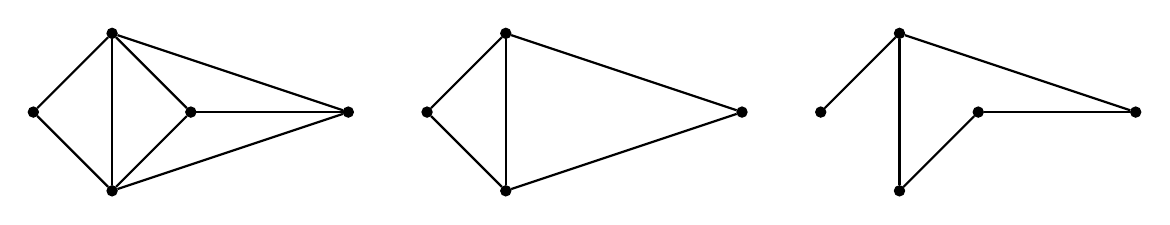
\begin{tikzpicture}

      \tikzset{enclosed/.style={draw, circle, inner sep=0pt, minimum size=.13cm, fill=black}}
% Vertices
	%Hel graf
      	\node[enclosed] (v1) at (0,2) {};
      	\node[enclosed] (v2) at (1,3) {};
    	\node[enclosed] (v3) at (1,1) {};
  	    \node[enclosed] (v4) at (4,2) {};
  	    \node[enclosed] (v5) at (2,2) {};
	%Induceret graf
		\node[enclosed] (v6) at (5,2) {};
      	\node[enclosed] (v7) at (6,3) {};
  	    \node[enclosed] (v8) at (6,1) {};
  	    \node[enclosed] (v9) at (9,2) {};
	%Udspændende graf
		\node[enclosed] (v10) at (10,2) {};
      	\node[enclosed] (v11) at (11,3) {};
   	 	\node[enclosed] (v12) at (11,1) {};
  	    \node[enclosed] (v13) at (14,2) {};
  	    \node[enclosed] (v14) at (12,2) {};
%Edges
	%Hel graf
		\path[thick] (v1) edge node {} (v2);
		\path[thick] (v1) edge node {} (v3);
		\path[thick] (v3) edge node {} (v4);
		\path[thick] (v3) edge node {} (v5);
		\path[thick] (v4) edge node {} (v5);
		\path[thick] (v2) edge node {} (v4);
		\path[thick] (v2) edge node {} (v5);
		\path[thick] (v2) edge node {} (v3);
	%Induceret graf
		\path[thick] (v6) edge node {} (v7);
		\path[thick] (v6) edge node {} (v8);
		\path[thick] (v8) edge node {} (v9);
		\path[thick] (v7) edge node {} (v9);
		\path[thick] (v7) edge node {} (v8);
	%Udspændende graf
		\path[thick] (v10) edge node {} (v11);
		\path[thick] (v11) edge node {} (v12);
		\path[thick] (v12) edge node {} (v14);
		\path[thick] (v14) edge node {} (v13);
		\path[thick] (v11) edge node {} (v13);

	\end{tikzpicture}
	\caption{Simpel graf, $G$ (venstre). Induceret delgraf af $G$ (midten). Udspændende delgraf af $G$ (højre).}
	\label{fig:delgraf.eks}
\end{figure}



\begin{defn}[\emph{k}-delt] \label{defn:k-delt} %k-partite
En graf, $G = (V, E)$, kaldes en \emph{$k$-delt graf}, hvis $V$ kan deles op i $k$ ikke-tomme delmængder, $V_1, V_2,\dotsc, V_k$, således at $V= V_1 \bigcup V_2 \bigcup \dotsc \bigcup V_k$. Foruden gælder det at $V_i \bigcap V_j  = \emptyset \forall i,j$, og $i\neq j$. Samtidigt kan to vilkårlige knuder, $v$ og $u$, kun være naboer, hvis de befinder sig i forskellige delmængder. 
\end{defn}


En af fordelene ved at dele en graf op i forskellige delgrafer er, at man i korteste vej-problemer kan finde den optimale delstruktur, hvis den optimale delgraf er fundet. 

Hvis man betragter \autoref{fig:laengste.vej}, kan man beskrive den korteste vej $P=(v_1,v_3,v_4)$ som en optimal delgraf. Denne delgraf har også en optimal delstruktur, da den korteste vej fra $v_1$ til $v_3$ indgår i vejen $P=(v_1,v_3,v_4)$.
Hvis vi kigger på den længste vej fra $v_1$ til $v_4$, $P=(v_1,v_3,v_4)$, ser vi, at den ikke har en optimal delstruktur, da den længste vej fra $v_1$ til $v_3$ ikke indgår i den længste vej fra $v_1$ til $v_4$.








